\documentclass[10pt,a4paper]{article}

\usepackage[margin=2.1cm]{geometry}
\usepackage{graphicx}
\usepackage{booktabs}
\usepackage{amsmath}
\usepackage[dvipsnames]{xcolor}
\usepackage{titlesec}
\usepackage[T1]{fontenc}
\usepackage{helvet}
\usepackage{caption}

\renewcommand{\familydefault}{\sfdefault}
\captionsetup{font=small, labelfont=bf, skip=4pt}
\titleformat{\section}{\large\bfseries}{\thesection}{0.6em}{}
\titlespacing{\section}{0pt}{10pt}{4pt}
\setlength{\parindent}{0pt}
\setlength{\parskip}{4pt}
\pagestyle{empty}

\definecolor{rule}{gray}{0.75}
\newcommand{\van}{\textsc{vanilla}}
\newcommand{\mix}{\textsc{mmix}}

\begin{document}

{\LARGE\bfseries Uniform vs.\ heterogeneous alphabets}\\[2pt]
{\large\color{gray} Breaking Assumption 1(iii) at matched total rate}\\[6pt]
{\footnotesize DDMS simulator $\cdot$ Gaussian shift, $p=1/2$ $\cdot$ exact error probability, no Monte Carlo}

\vspace{2pt}
{\color{rule}\hrule height 0.6pt}
\vspace{6pt}

\section*{Setup}

Two schemes spend an identical communication budget of $R$ bits.
\van{} is the article's setting: every sensor uses the same $M=4$
quantizer, $2$ bits each, so $|U^i|$ is uniform and Assumption 1(iii)
holds. \mix{} gives a fraction $c$ of the sensors a $1$-bit $M=2$
quantizer and the rest the $M=4$ one, so alphabets differ across
sensors and the assumption fails. Thresholds are nested,
$\{1\} \subset \{0.2, 1, 5\}$, so alphabet size is the only variable.

Matching the budget fixes the sensor count: $N = R/(2-c)$. Spending
bits on coarser sensors therefore buys \emph{more} of them --- at
$R=240$, \van{} fields $120$ sensors and all-$1$-bit fields $240$.
The metric is the total error exponent $-\log J^{N}$; each $2.3$ units
is one more decimal place of reliability.

\begin{figure}[h]
\centering
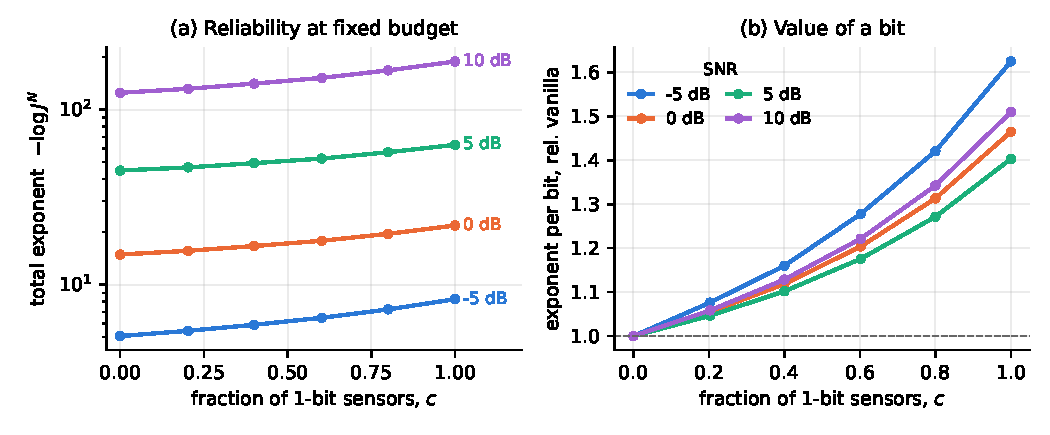
\includegraphics[width=\textwidth]{fig_report_gain.pdf}
\caption{At $R=240$ bits. (a) Exponent rises monotonically as budget
shifts to $1$-bit sensors, at every SNR. (b) The same effect per bit:
a bit is worth $1.4$--$1.6\times$ more when spent on a new sensor than
on finer resolution.}
\end{figure}

\section*{Results at $R = 240$ bits}

\begin{center}
\small
\begin{tabular}{lrrrr}
\toprule
& \multicolumn{4}{c}{SNR} \\
\cmidrule(l){2-5}
& $-5$ dB & $0$ dB & $5$ dB & $10$ dB \\
\midrule
\van{} exponent ($c=0$, $N=120$)      & 5.08 & 14.85 & 44.83 & 124.64 \\
\mix{} exponent ($c=0.6$, $N=171$)    & 6.47 & 17.80 & 52.49 & 151.62 \\
All $1$-bit ($c=1$, $N=240$)          & 8.25 & 21.75 & 62.90 & 188.14 \\
\midrule
Error reduction, $c=0 \to 1$          & $10^{1.4}\times$ & $10^{3.0}\times$ & $10^{7.8}\times$ & $10^{27.6}\times$ \\
Mixing penalty (exact/average)        & \multicolumn{4}{c}{$0.997$--$1.024$ over all $48$ mixed banks} \\
\bottomrule
\end{tabular}
\end{center}

\begin{figure}[h]
\centering
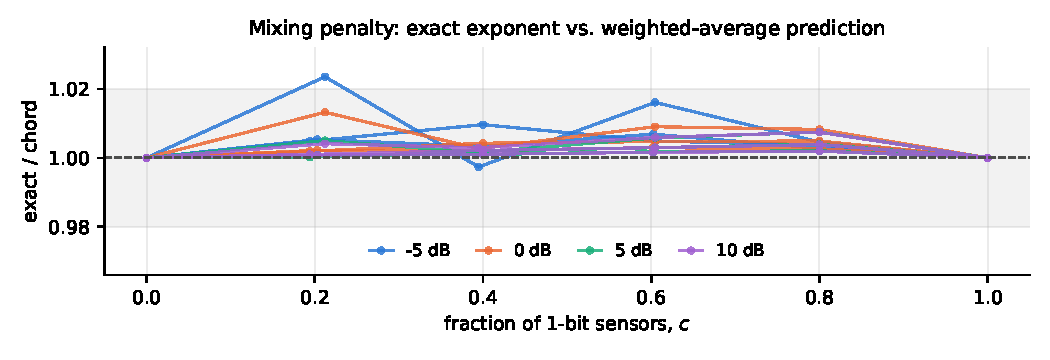
\includegraphics[width=\textwidth]{fig_report_chord.pdf}
\caption{Every mixed bank, all four SNRs and all three budgets
($60/120/240$ bits), against the weighted average of the two uniform
endpoints. Deviations stay inside $\pm 2\%$ and shrink as the budget
grows: heterogeneity itself is free.}
\end{figure}

\section*{\van{} --- uniform $|U|=4$}

\textbf{Pros.} Inside Assumption 1(iii), so the article's exponent
results apply directly. Exchangeable sensors give the cheapest exact
computation (one multinomial). Fewest sensors for a given budget ---
the right choice when hardware, not bandwidth, is the binding
constraint.

\textbf{Cons.} Weakest configuration per bit at every SNR tested. The
second bit only refines confidence, while a first bit buys an
independent opinion; at $R=240$, $0$ dB it gives up a factor $10^{3}$
in error probability against the same budget spent on $1$-bit sensors.

\section*{\mix{} --- heterogeneous $|U| \in \{2,4\}$}

\textbf{Pros.} Strictly better exponent than \van{} at equal budget,
tunable continuously through $c$. Costs nothing beyond the
reallocation itself --- performance is the rate-weighted average of
the uniform schemes to within $2\%$. Practical when sensors are
genuinely unequal (different hardware, links, or battery), since a
mixed fleet loses no efficiency.

\textbf{Cons.} Outside Assumption 1(iii), so the article's analysis
does not formally cover it. Needs more sensors and a fusion center
that tracks per-sensor $\gamma^i$. Exact evaluation is costlier
(cross-group convolution). And the gain is not from heterogeneity:
the uniform all-$1$-bit bank is better still.

\section*{Conclusions}

\textbf{1. Assumption 1(iii) is a proof convenience, not a
performance boundary.} Mixed banks land on the straight line between
uniform ones. Given the hypothesis, sensors are independent and their
log-likelihood contributions simply add --- the fusion center is
indifferent to whether they came from matching alphabets.

\textbf{2. The real lever is rate allocation, not uniformity.} Under
a bit budget, more coarse sensors beat fewer fine ones at every SNR:
$1$-bit sensors convert bits into exponent $1.4$--$1.6\times$ more
efficiently. The effect strengthens with SNR, where a single
threshold already separates the hypotheses well.

\textbf{3. Read exponents as digits of reliability.} Because errors
decay exponentially, the modest gap $14.85 \to 21.75$ at $0$ dB is
three orders of magnitude in $J^{N}$.

\vspace{2pt}
{\color{rule}\hrule height 0.4pt}
\vspace{3pt}
{\footnotesize\color{gray} Caveat: measured at fixed nested thresholds
$\{0.2,1,5\}$. Whether $M=4$ with Chernoff-optimized thresholds closes
the per-bit gap is untested. Static heterogeneity only --- alphabets
are fixed in advance, not adapted to observations. Source:
\texttt{runs/Mmix/csweep\_M2M4\_*\_2026-08-03}.}

\end{document}
